%!TEX TS-program = pdflatex
%!TEX root = ../main.tex
%!TEX encoding = UTF-8 Unicode


\section[Application]{Application}

\subsection[System design]{System design}

\begin{frame}{Use Case Diagram}
	The first step of our development to identify the use cases of our system.
	We have identified four main use cases:

	\begin{figure}[h!]
		\centering
		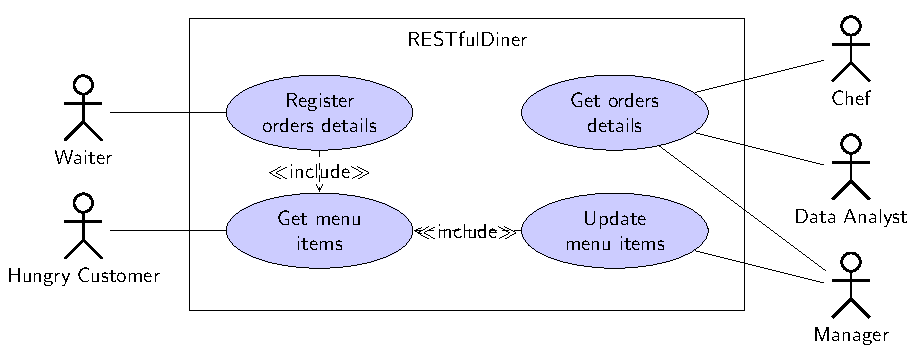
\includegraphics[width=0.9\textwidth,height=0.55\textheight,keepaspectratio]{images/usecases}
		\vspace*{-1\baselineskip}
		\caption{Use cases diagram}
		\label{fig:usecases}
	\end{figure}

\end{frame}

\begin{frame}{E/R Diagram}
	Next, the E/R diagram was designed to represent the data model of the
	system:

	\begin{figure}[h!]
		\centering
		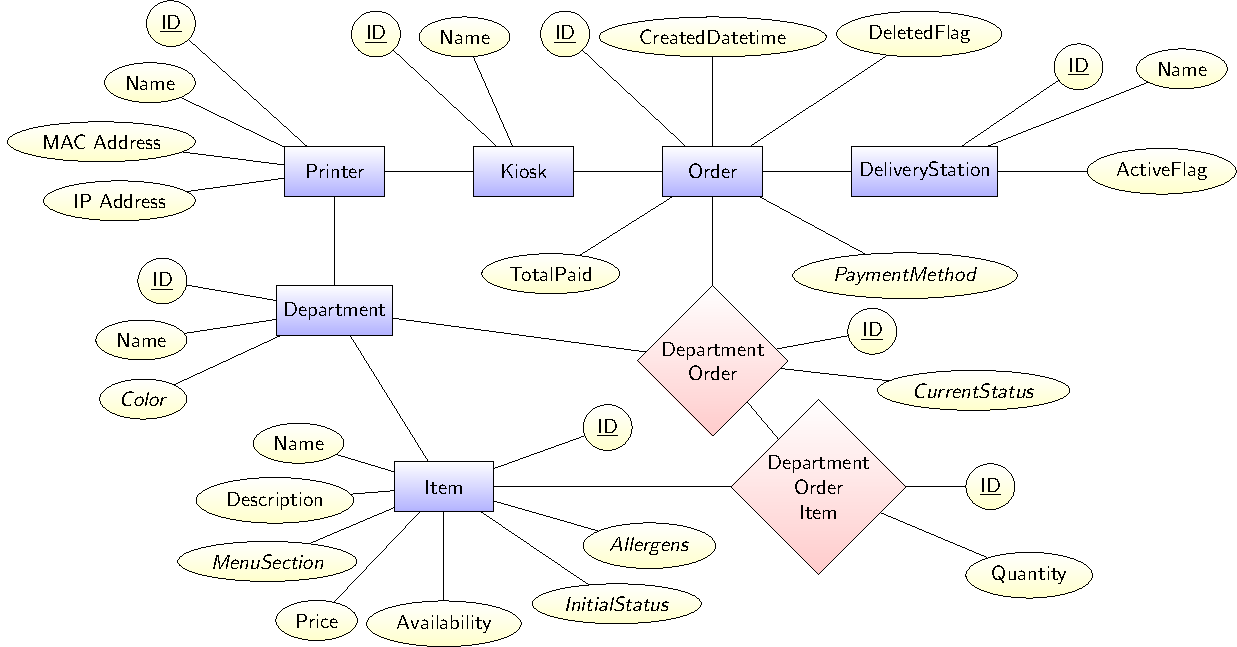
\includegraphics[width=\textwidth,height=0.6\textheight,keepaspectratio]{images/er}
		\caption{E/R diagram}
		\label{fig:er}
	\end{figure}

\end{frame}

\subsection[System implementation]{System implementation}

\begin{frame}[allowframebreaks]{Data model implementation}

	The data model has been implemented using the SQLAlchemy ORM, which
	provides a high-level interface to the (PostgreSQL, in this case) database.

	\lstinputlisting[language=PythonPlus,linerange={18-28}]{../app/models/_base.py}

	Any class inherits from the \texttt{BaseModel} class and is automatically
	mapped to a table in the database.

	\framebreak

	\vspace*{-1\baselineskip}
	\lstinputlisting[language=PythonPlus,linerange={17-38}]{../app/models/department.py}

\end{frame}

\begin{frame}[allowframebreaks,fragile]{API resources}
	The RESTful API has been implemented using the Flask web framework.

	\lstinputlisting[language=PythonPlus,linerange={12-12,16-33}]{../app/resources/department.py}

	\framebreak

	\begin{lstlisting}[caption={\texttt{GET /api/v1/departments/851c8de8-fb55-11ef-9aea-0242ac120003} response}]
	"@context": {
		"schema": "https://schema.org/",
		"self": "@id",
		"type": "@type",
		"name": "schema:name",
		"printer": {
			"@id": "schema:isRelatedTo",
			"@type": "@id"
		},
		"license": {
			"@id": "schema:license",
			"@type": "@id"
		}
	},
	"license": "https://creativecommons.org/licenses/by/4.0/",
	"self": "http://127.0.0.1/api/v1/departments/851c8de8-fb55-11ef-9aea-0242ac120003",
	"type": "schema:Organization",
	"name": "Kitchen",
	"printer": "http://127.0.0.1/api/v1/printers/67936882-fb55-11ef-b5b9-0242ac120003"\end{lstlisting}

\end{frame}

\begin{frame}{Demo}
	A live demo of the system is available at \url{https://diner.enricostefanel.it}.

	\begin{figure}
		\centering
		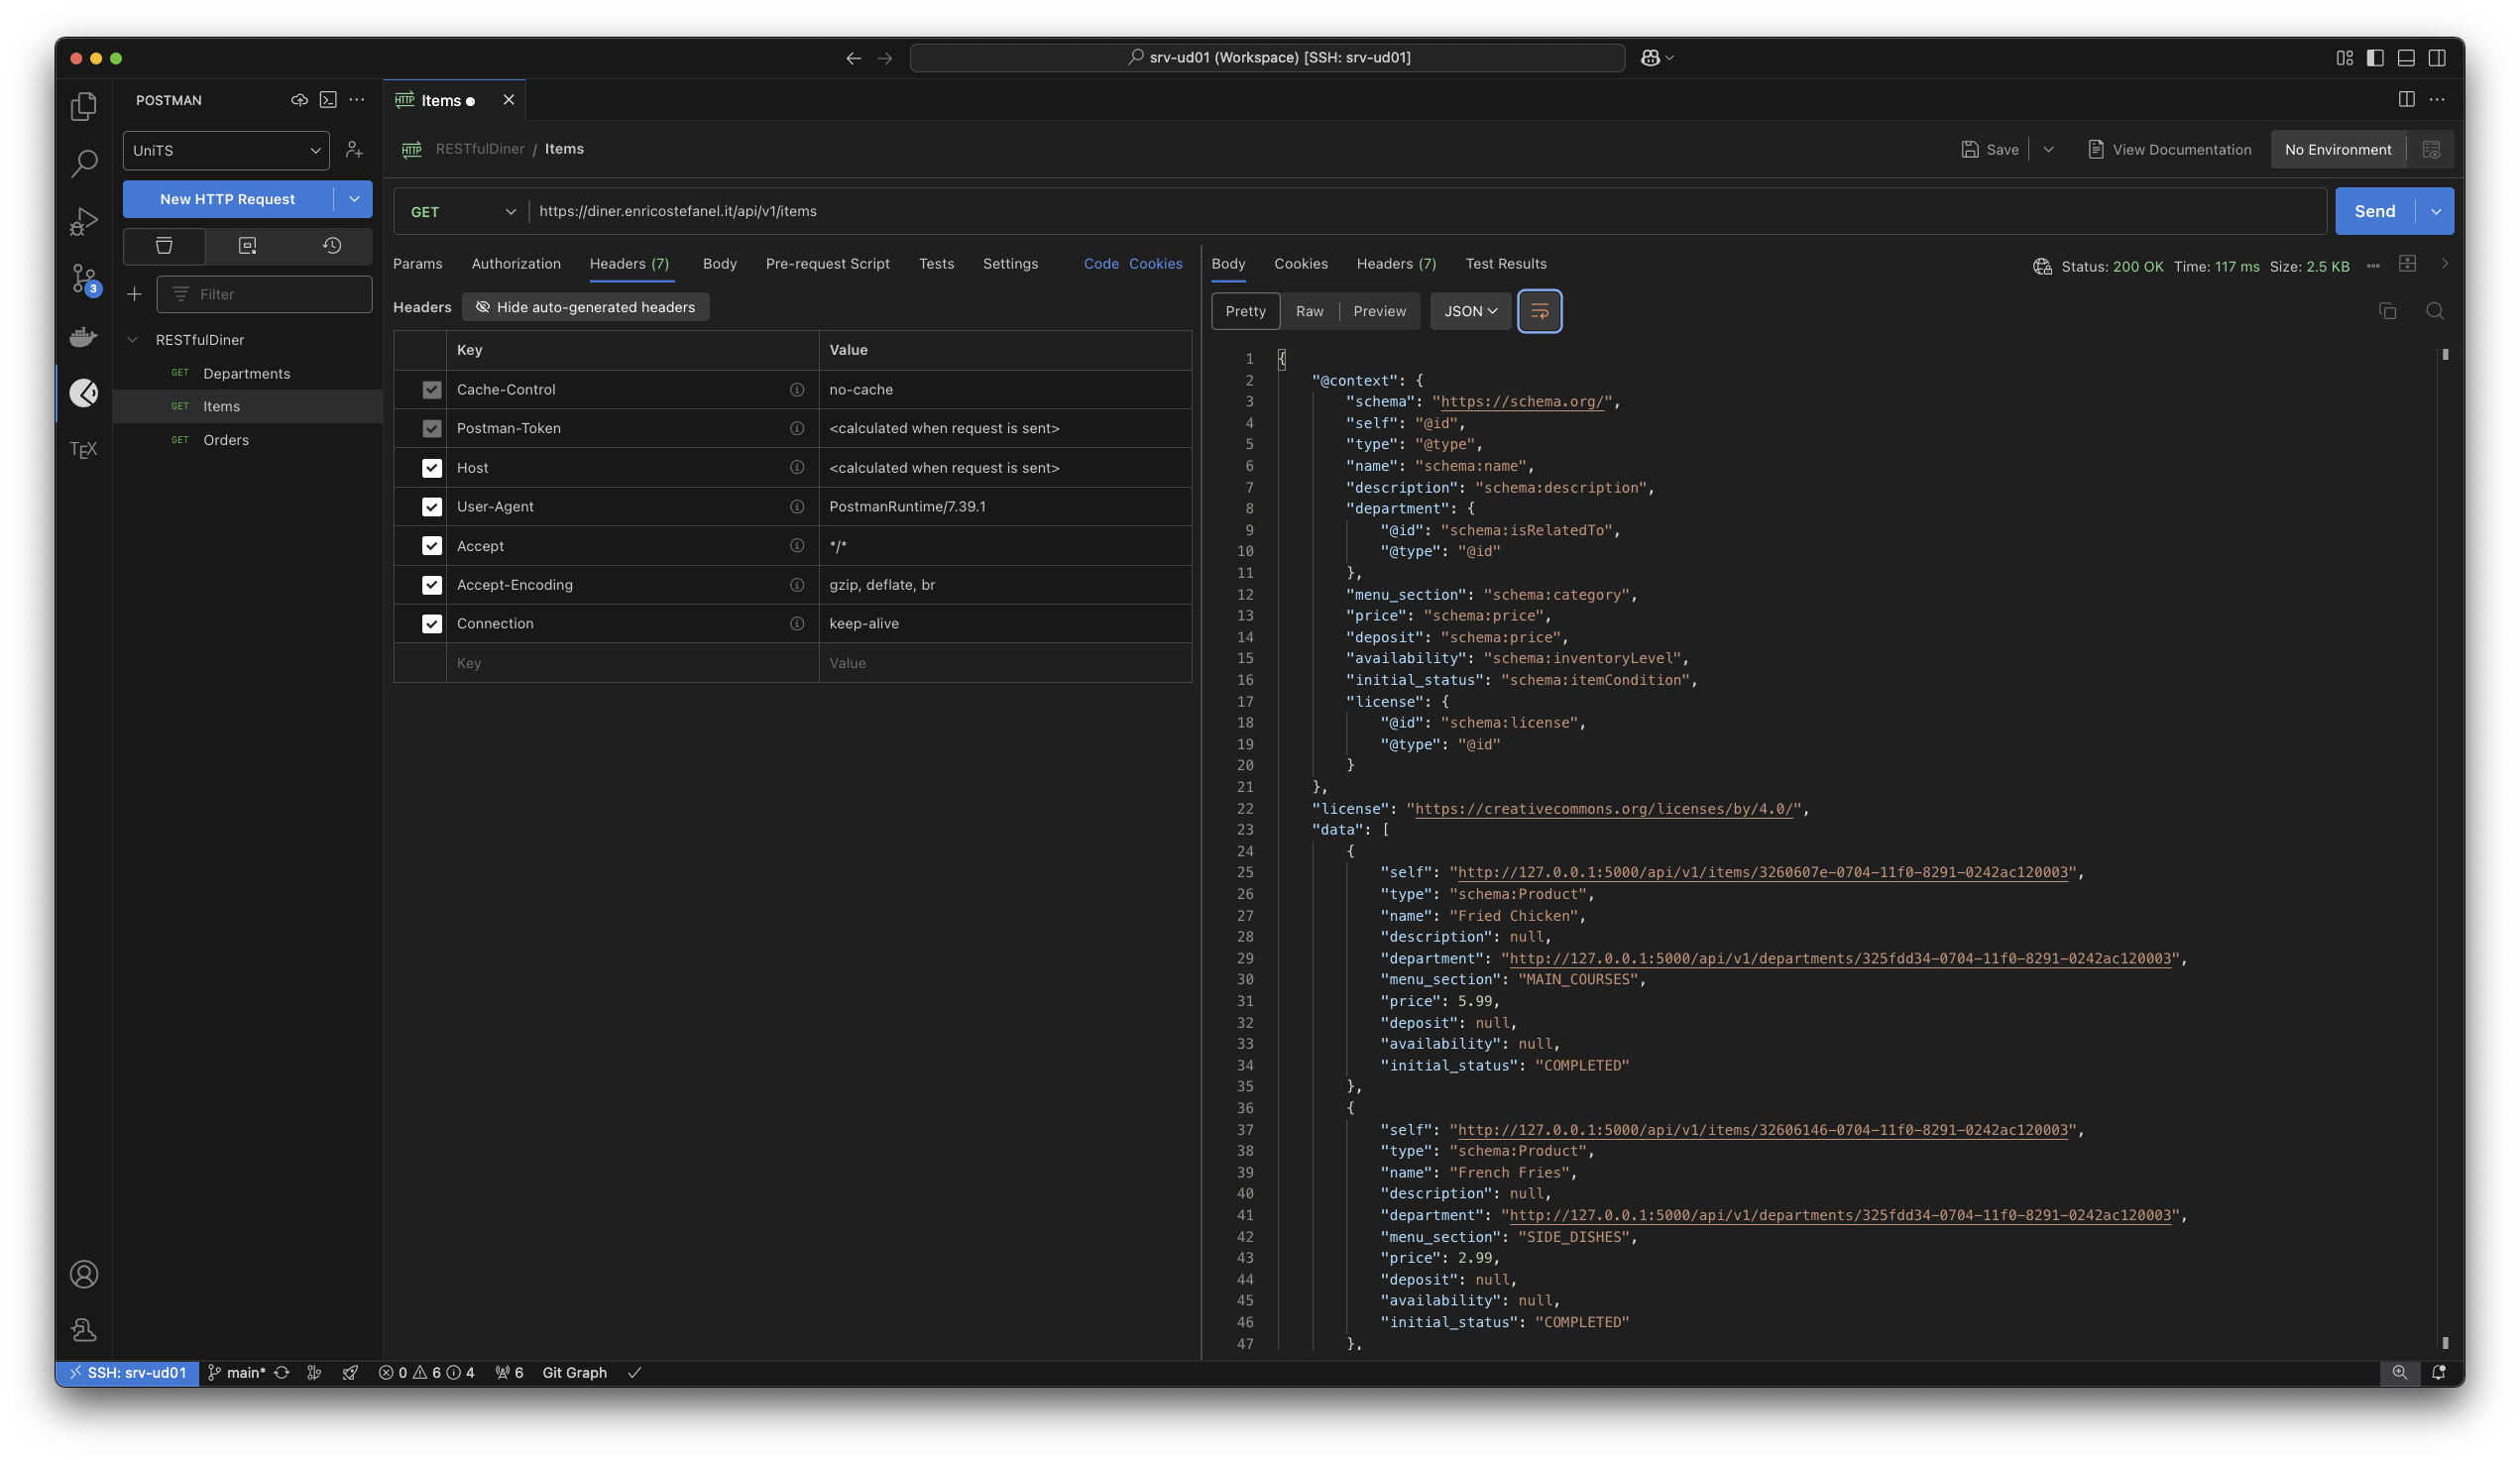
\includegraphics[width=0.9\textwidth,height=0.6\textheight,keepaspectratio]{images/postman.png}
		\vspace*{-1\baselineskip}
		\caption{Demo of the system using Postman}
		\label{fig:demo}
	\end{figure}
\end{frame}


\section[Open Data principles]{Open Data principles}

\subsection[Linked Open Data]{Linked Open Data}

\begin{frame}[allowframebreaks]{Linked Open Data\autocite{Berners-Lee_2006} requirements}
	\begin{block}{\faStar\faStarO\faStarO\faStarO\faStarO}
		Make your stuff available on the Web (whatever format) under an open
		license.
	\end{block}
	\vspace*{-8pt}
	\begin{block}{\faStar\faStar\faStarO\faStarO\faStarO}
		Make it available as structured data (e.g., Excel instead of image scan
		of a table).
	\end{block}
	\vspace*{-8pt}
	\begin{block}{\faStar\faStar\faStar\faStarO\faStarO}
		Make it available in a non-proprietary open format (e.g., CSV instead of
		Excel).
	\end{block}
	These requirements are satisfied by our RESTful API that allows
	publicly access to data in JSON-LD\autocite{Sporny_2014} format and provide
	them under Creative Commons license.

	\framebreak

	\begin{block}{\faStar\faStar\faStar\faStar\faStarO}
		Use URIs to denote things, so that people can point at your stuff.
	\end{block}
	\vspace*{-8pt}
	\begin{block}{\faStar\faStar\faStar\faStar\faStar}
		Link your data to other data to provide context.
	\end{block}
	Every resource in the system is identified by a URI, and can be accessed
	by a simple HTTP GET request to that URI. A relation between resources
	is established by linking them in the JSON response.
\end{frame}


\subsection[Data Management]{Data Management}

\begin{frame}[allowframebreaks]{Data Management Plan}

	\begin{enumerate}
		\item \textbf{How will the data be created?} The data will be created by the
		      restaurant staff, who will use the system to manage the restaurant's
		      departments, tables, and printers.
		\item \textbf{How will the data be documented?} The data will be documented in
		      the system's database, and the API will provide a JSON-LD representation of
		      the data.
		\item \textbf{Who will access the data?} The data will be publicly accessible
		      through the RESTful API.
		\item \textbf{How will the data be stored?} The data will be stored by the
		      system's database, which is a PostgreSQL database. In case, the database
			  can also be installed on a cloud service.
		\item \textbf{How will the data be shared?} The data will be shared through the
		      RESTful API, which will provide a JSON-LD representation of the data for
			  basic HTTP requests (GET, POST, PUT, DELETE).
		\item \textbf{How will the data be preserved?} The data will be preserved by
		      the system's database, which will be backed up regularly to ensure data
			  integrity.
		\item \textbf{Who will back up the data?} The data will be backed up by the
		      system administrator, who will ensure that the database is backed up
			  regularly.
	\end{enumerate}
\end{frame}
